\chapter{Revisão Bibliográfica}

% Para ilustrar a completa ades\~ao ao estilo de cita{\c c}\~oes e listagem de
% refer\^encias bibliogr\'aficas, a Tabela~\ref{tab:citation} apresenta cita{\c
% c}\~oes de alguns dos trabalhos contidos na norma fornecida pela CPGP da
% COPPE, utilizando o estilo num\'erico.
% 
% \begin{table}[h]
% \caption{Exemplos de cita{\c c}\~oes utilizando o comando padr\~ao
%   \texttt{\textbackslash cite} do \LaTeX\ e
%   o comando \texttt{\textbackslash citet},
%   fornecido pelo pacote \texttt{natbib}.}
% \label{tab:citation}
% \centering
% {\footnotesize
% \begin{tabular}{|c|c|c|}
%   \hline
%   Tipo da Publica{\c c}\~ao & \verb|\cite| & \verb|\citet|\\
%   \hline
%   Livro & \cite{book-example} & \citet{book-example}\\
%   Artigo & \cite{article-example} & \citet{article-example}\\
%   Relat\'orio & \cite{techreport-example} & \citet{techreport-example}\\
%   Relat\'orio & \cite{techreport-exampleIn} & \citet{techreport-exampleIn}\\
%   Anais de Congresso & \cite{inproceedings-example} &
%     \citet{inproceedings-example}\\
%   S\'eries & \cite{incollection-example} & \citet{incollection-example}\\
%   Em Livro & \cite{inbook-example} & \citet{inbook-example}\\
%   Disserta{\c c}\~ao de mestrado & \cite{mastersthesis-example} &
%     \citet{mastersthesis-example}\\
%   Tese de doutorado & \cite{phdthesis-example} & \citet{phdthesis-example}\\
%   \hline
% \end{tabular}}
% \end{table}

% -.~.-.~.-.~.-.~.-.~.-.~.-.~.-.~.-.~.-.~.-.~.-
\section{Dinâmica de Sistemas Multicorpos}

\subsection{Cinemática}\label{sec::cinematica}

\subsection{Cinemática Inversa e planejamento de
trajetória}\label{sec::ikin_traj}

\subsection{Dinâmica}

\subsection{Equações de Movimento}

\subsection{Sophia-Maple e Método de Kane}\label{sec::sophia-kane}

\subsubsection{Notação de Lesser e Lennartsson}


% -.~.-.~.-.~.-.~.-.~.-.~.-.~.-.~.-.~.-.~.-.~.-
\section{Análise dinâmica de estruturas}

\subsection{Matriz de rigidez} \label{sec::rigidez}

\subsection{Amortecimento proporcional} \label{sec::amortecimento}

\subsection{Frequência Natural, Modo de Vibração e Amortecimento}
\label{sec::param_mod}

\subsection{Ensaio experimental de vibrações}


% -.~.-.~.-.~.-.~.-.~.-.~.-.~.-.~.-.~.-.~.-.~.-
\section{Manipuladores robóticos industriais}\label{sec::manind}

\subsection{Manipuladores flexíveis}

\subsection{Manipuladores sobre bases flexíveis}

\subsection{Tarefas de precisão utilizando manipuladores robóticos}

\subsection{Sistema de revestimento por asperção térmica} \label{sec::hvof}

\subsection{Tarefas robóticas \textit{in-situ}} \label{sec::insitu}

\lipsum[1-1]

\begin{figure}[h]
	\centering 
 	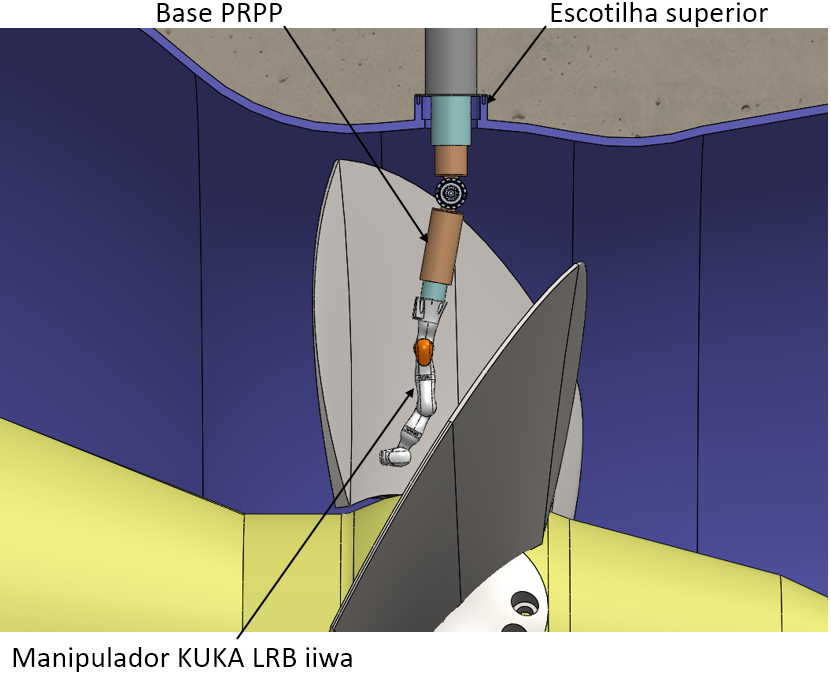
\includegraphics[width=0.85\textwidth]{figs/base_telesc_turbina}
 	\caption{Base telescópica PRP para manutenção de revestimento
 	\textit{in-situ}}
 	\label{fig::base_telesc_turbina}
\end{figure}

\begin{figure}[h]
	\centering 
 	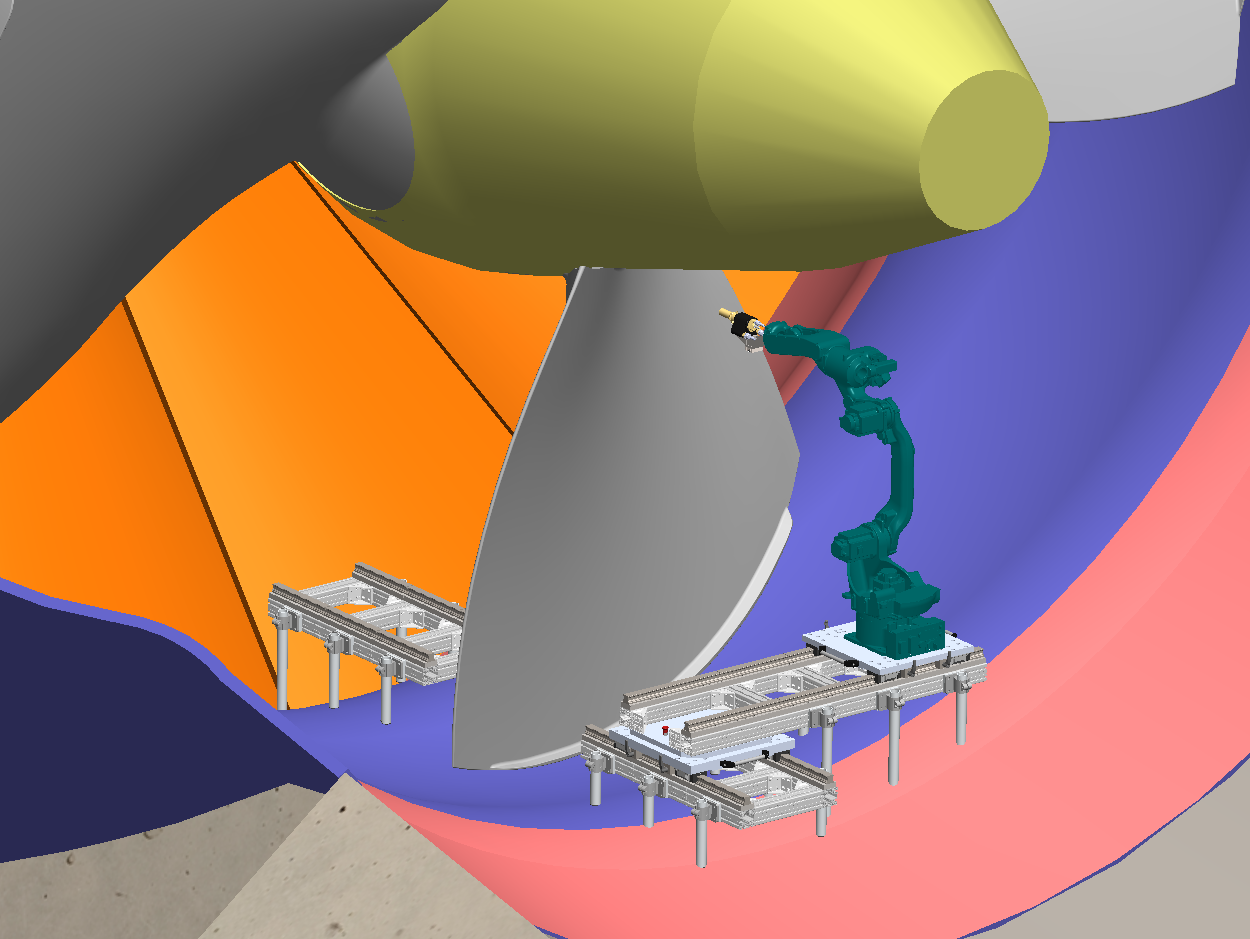
\includegraphics[width=0.85\textwidth]{figs/prp_turbina}
 	\caption{Base modular PRP para manutenção de revestimento \textit{in-situ}}
 	\label{fig::prp_turbina}
\end{figure}




















